\documentclass[a4paper,10pt]{article}
\usepackage{graphicx}
\usepackage{float}
\usepackage{fancyhdr}
%\usepackage{vmargin}

\title{ Data Mining}								
\makeatletter
\let\thetitle\@title
\makeatother

\pagestyle{fancy}
\fancyhf{}
\cfoot{\thepage}

\begin{document}

%%%%%%%%%%%%%%%%%%%%%%%%%%%%%%%%%%%%%%%%%%%%%%%%%%%%%%%%%%%%%%%%%%%%%%%%%%%%%%%%%%%%%%%%%

\begin{titlepage}
	\centering
    \vspace*{0.5 cm}
    
\includegraphics[scale = 0.75]{logo.jpg}\\[1.0 cm]	% University Logo
    \textsc{\LARGE \bfseries Bangabandhu Sheikh Mujibur Rahaman Science and Technology University}\\[1 cm]	% University Name
	\textsc{\LARGE \bfseries REPORT}\\[0.5 cm]
	\textsc{\Large \bfseries On}\\[0.5 cm]
	\rule{\linewidth}{0.2 mm} \\[0.4 cm]
	{ \huge \bfseries \thetitle}\\
	\rule{\linewidth}{0.2 mm} \\[0.5 cm]
	\textsc{\LARGE \bfseries Course Code: \large CSE-156}\\[0.5 cm]
	
	\begin{minipage}{0.4\textwidth}
		\begin{flushleft} \large
			\emph{\LARGE \bfseries Submitted By:}\\
			\Large Ashiq Ibne Shafi\\
             18ICTCSE047\\
            Dep. of CSE\\
            Sheikh Hasina Institute of ICT,BSMRSTU\\
			\end{flushleft}
			\end{minipage}~
			\begin{minipage}{0.5\textwidth}
            
			\begin{flushright} \large
			\emph{\LARGE \bfseries Submitted To:} \\
			 Nasif Ahmed\\
            Lecturer\\
            Dep. of CSE\\
     
		\end{flushright}
        
	\end{minipage}\\[2 cm]
	
	
    \emph{\LARGE Date of Submission: 23-01-2020}\\
    
    
    
	
\end{titlepage}

 %front matter stuff
    \pagenumbering{roman}
    \section*{Summary}
    \addcontentsline{toc}{section}{\numberline{}Summary}
 Data Mining is all about explaining the past and predicting the future for analysis. Data mining helps to extract information from huge sets of data. It is the procedure of mining knowledge from data. Data mining process includes business understanding, Data Understanding, Data Preparation, Modelling, Evolution, Deployment. Important Data mining techniques are Classification, clustering, Regression, Association rules, Outer detection, Sequential Patterns, and prediction. R-language and Oracle Data mining are prominent data mining tools. Data mining technique helps companies to get knowledge-based information.The main drawback of data mining is that many analytics software is difficult to operate and requires advance training to work on. Data mining is used in diverse industries such as Communications, Insurance, Education, Manufacturing, Banking, Retail, Service providers, eCommerce, Supermarkets Bioinformatics.
    \cleardoublepage

    %table of contents
    \tableofcontents
    \thispagestyle{empty}
    \cleardoublepage

    %main body stuff
    \pagenumbering{arabic}
    \setcounter{page}{1}

\section{introduction}\label{sec:intro}
Data mining is looking for hidden, valid, and potentially useful patterns in huge data sets. Data Mining is all about discovering
unsuspected/ previously unknown relationships amongst the data.It is a multi-disciplinary skill that uses machine learning, statistics, AI and database technology.The insights derived via Data Mining can be used for marketing, fraud detection, and scientific discovery, etc.
Data mining is also called as Knowledge discovery, Knowledge extraction, data/pattern analysis, information harvesting, etc.

\section{What is Data Mining?}

The process of extracting information to identify patterns, trends, and useful data that would allow the business to take the data-driven decision from huge sets of data is called Data Mining.

In other words, we can say that Data Mining is the process of investigating hidden patterns of information to various perspectives for categorization into useful data, which is collected and assembled in particular areas such as data warehouses, efficient analysis, data mining algorithm, helping decision making and other data requirement to eventually cost-cutting and generating revenue.

Data mining is the act of automatically searching for large stores of information to find trends and patterns that go beyond simple analysis procedures. Data mining utilizes complex mathematical algorithms for data segments and evaluates the probability of future events. Data Mining is also called Knowledge Discovery of Data (KDD).

Data Mining is a process used by organizations to extract specific data from huge databases to solve business problems. It primarily turns raw data into useful information.

Data Mining is similar to Data Science carried out by a person, in a specific situation, on a particular data set, with an objective. This process includes various types of services such as text mining, web mining, audio and video mining, pictorial data mining, and social media mining. It is done through software that is simple or highly specific. By outsourcing data mining, all the work can be done faster with low operation costs. Specialized firms can also use new technologies to collect data that is impossible to locate manually. There are tonnes of information available on various platforms, but very little knowledge is accessible. The biggest challenge is to analyze the data to extract important information that can be used to solve a problem or for company development. There are many powerful instruments and techniques available to mine data and find better insight from it.

\begin{figure}[H]
	\centering
	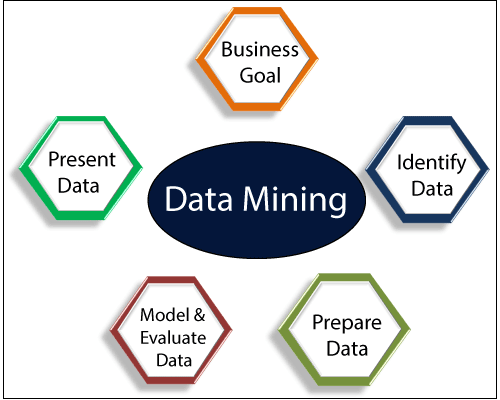
\includegraphics[width=\linewidth]{DIntro.png}
\end{figure}

\section{Types Of Data}
Data mining can be performed on following types of data:
\begin{itemize}
	\item Relational databases
	\item Data warehouses
	\item Advanced DB and information repositories
	\item Object-oriented and object-relational databases
	\item Transactional and Spatial databases
	\item Heterogeneous and legacy databases
	\item Multimedia and streaming database
	\item Text databases
	\item Text mining and Web mining
\end{itemize}
\newpage
\section{Data Mining Implementation Process}

\begin{figure}[H]
           \centering
           
\includegraphics[width=\linewidth]{figure1.png}

\end{figure}
Let's study the Data Mining implementation process in detail
\subsection{Business understanding:}
In this phase, business and data-mining goals are established.
\begin{itemize}
	\item First, you need to understand business and client objectives. You need to define what your client wants (which many times even they do not know themselves)
	\item Take stock of the current data mining scenario. Factor in resources, assumption, constraints, and other significant factors into your assessment.
	\item Using business objectives and current scenario, define your data mining goals.
	\item A good data mining plan is very detailed and should be developed to accomplish both business and data mining goals.
\end{itemize}

\subsection{Data understanding:}
In this phase, sanity check on data is performed to check whether its appropriate for the data mining goals.
\begin{itemize}
	\item First, data is collected from multiple data sources available in the organization.
	\item These data sources may include multiple databases, flat filer or data cubes. There are issues like object matching and schema.
	\item Therefore, it is quite difficult to ensure that both of these given objects refer to the same value or not. Here, Metadata should be used to reduce errors in the data integration process.
	\item Next, the step is to search for properties of acquired data. A good way to explore the data is to answer the data mining questions (decided in business phase) using the query, reporting, and visualization tools.
	\item Based on the results of query, the data quality should be ascertained. Missing data if any should be acquired.
\end{itemize}
\newpage
\subsection{Data transformation:}
Data transformation operations would contribute toward the success of the mining process.
\subsection*{Smoothing:It helps to remove noise from the data.}
\subsection*{Aggregation: \small Summary or aggregation operations are applied to the data. I.e., the weekly sales data is aggregated to calculate the monthly and yearly total.}
\subsection*{Generalization: \small In this step, Low-level data is replaced by higher-level concepts with the help of concept hierarchies. For example, the city is replaced by the county.}
\subsection*{Normalization: \small Normalization performed when the attribute data are scaled up o scaled down. Example: Data should fall in the range -2.0 to 2.0 post-normalization.}
\subsection*{Attribute construction: \small These attributes are constructed and included the given set of attributes helpful for data mining.}

The result of this process is a final data set that can be used in modeling.

\subsection{Modelling:}
In this phase, mathematical models are used to determine data patterns.
\begin{itemize}
	\item Based on the business objectives, suitable modeling techniques should be selected for the prepared dataset.
	\item Create a scenario to test check the quality and validity of the model.
	\item Run the model on the prepared dataset.
	\item Results should be assessed by all stakeholders to make sure that model can meet data mining objectives.
\end{itemize}

\subsubsection{Evaluation:}
In this phase, patterns identified are evaluated against the business objectives.
\begin{itemize}
	\item Results generated by the data mining model should be evaluated against the business objectives.
	\item Gaining business understanding is an iterative process. In fact, while understanding, new business requirements may be raised because of data mining.
	\item go or no-go decision is taken to move the model in the deployment phase.
\end{itemize}

\subsubsection{Deployment:}
In the deployment phase, you ship your data mining discoveries to everyday business operations.
\begin{itemize}
	\item The knowledge or information discovered during data mining process should be made easy to understand for non-technical stakeholders.
	\item A detailed deployment plan, for shipping, maintenance, and monitoring of data mining discoveries is created.\\
	\item A final project report is created with lessons learned and key experiences during the project. This helps to improve the organization's business policy.
\end{itemize}
\section{Challenges of Implementation in Data mining:}

Although data mining is very powerful, it faces many challenges during its execution. Various challenges could be related to performance, data, methods, and techniques, etc. The process of data mining becomes effective when the challenges or problems are correctly recognized and adequately resolved.

\begin{figure}[H]
	\centering
	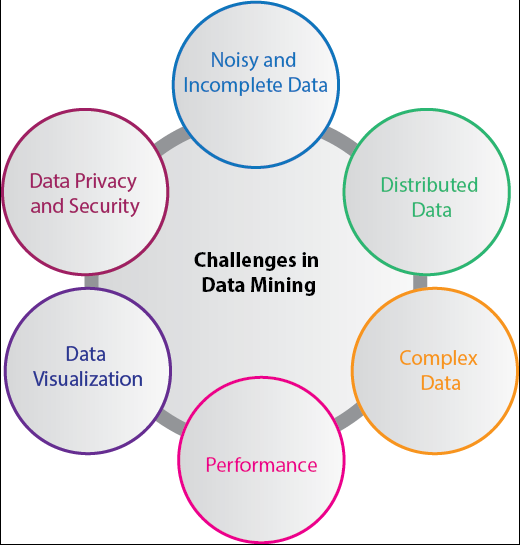
\includegraphics[width=\linewidth]{CData.png}
\end{figure}
\newpage
\subsection{Incomplete and noisy data:}


The process of extracting useful data from large volumes of data is data mining. The data in the real-world is heterogeneous, incomplete, and noisy. Data in huge quantities will usually be inaccurate or unreliable. These problems may occur due to data measuring instrument or because of human errors. Suppose a retail chain collects phone numbers of customers who spend more than 500, and the accounting employees put the information into their system. The person may make a digit mistake when entering the phone number, which results in incorrect data. Even some customers may not be willing to disclose their phone numbers, which results in incomplete data. The data could get changed due to human or system error. All these consequences (noisy and incomplete data)makes data mining challenging.

\subsection{Data Distribution:}

Real-worlds data is usually stored on various platforms in a distributed computing environment. It might be in a database, individual systems, or even on the internet. Practically, It is a quite tough task to make all the data to a centralized data repository mainly due to organizational and technical concerns. For example, various regional offices may have their servers to store their data. It is not feasible to store, all the data from all the offices on a central server. Therefore, data mining requires the development of tools and algorithms that allow the mining of distributed data.

\subsection{Complex Data:}

Real-world data is heterogeneous, and it could be multimedia data, including audio and video, images, complex data, spatial data, time series, and so on. Managing these various types of data and extracting useful information is a tough task. Most of the time, new technologies, new tools, and methodologies would have to be refined to obtain specific information.

\subsection{Performance:}

The data mining system's performance relies primarily on the efficiency of algorithms and techniques used. If the designed algorithm and techniques are not up to the mark, then the efficiency of the data mining process will be affected adversely.

\subsection{Data Privacy and Security:}

Data mining usually leads to serious issues in terms of data security, governance, and privacy. For example, if a retailer analyzes the details of the purchased items, then it reveals data about buying habits and preferences of the customers without their permission.

\subsection{Data Visualization:}

In data mining, data visualization is a very important process because it is the primary method that shows the output to the user in a presentable way. The extracted data should convey the exact meaning of what it intends to express. But many times, representing the information to the end-user in a precise and easy way is difficult. The input data and the output information being complicated, very efficient, and successful data visualization processes need to be implemented to make it successful.

\section{Data Mining Techniques}

\begin{figure}[H]
           \centering
           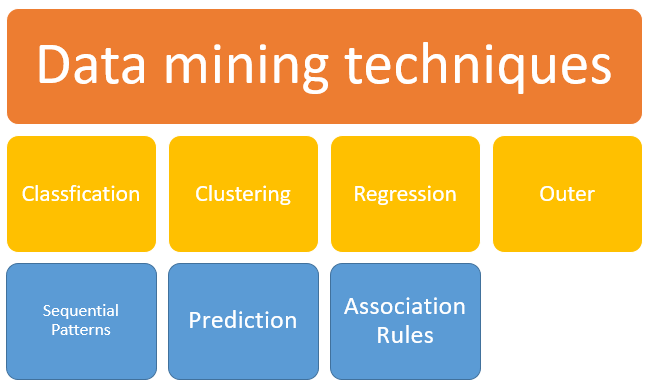
\includegraphics[width=\linewidth]{figure2.png}

\end{figure}

\subsection*{1.Classification:}
This analysis is used to retrieve important and relevant information about data, and metadata.This data mining method helps to classify data in different classes.

\subsection*{2. Clustering:}
Clustering analysis is a data mining technique to identify data that are like each other. This process helps to understand the differences and similarities between the data.

\subsection*{3. Regression:}
Regression analysis is the data mining method of identifying and analyzing the relationship between variables. It is used to identify the likelihood of a specific variable, given the presence of other variables.

\subsection*{4. Association Rules:}
This data mining technique helps to find the association between two or more Items. It discovers a hidden pattern in the data set.

\subsection*{5. Outer detection:}
This type of data mining technique refers to observation of data items in the dataset which do not match an expected pattern or expected behavior. This technique can be used in a variety of domains, such as intrusion, detection, fraud or fault detection, etc. Outer detection is also called Outlier Analysis or Outlier mining.

\subsection*{6. Sequential Patterns:}
This data mining technique helps to discover or identify similar patterns or trends in transaction data for certain period.

\subsection*{7. Prediction:}
Prediction has used a combination of the other data mining techniques like trends, sequential patterns, clustering, classification, etc. It analyzes past events or instances in a right sequence for predicting a future event.

\section{Data mining Examples:}
\subsection*{Example 1:}
Consider a marketing head of telecom service provides who wants to increase revenues of long distance services. For high ROI on his 
sales and marketing efforts customer profiling is important. He has a vast data pool of customer information like age, gender, income, credit history, etc. But its impossible to determine characteristics of people who prefer long distance calls with manual analysis. Using data mining techniques, he may uncover patterns between high long distance call users and their characteristics.

\subsection*{Example 2:}
A bank wants to search new ways to increase revenues from its credit card operations. They want to check whether usage would double if fees were halved.

Bank has multiple years of record on average credit card balances, payment amounts, credit limit usage, and other key parameters. They create a model to check the impact of the proposed new business policy.

\section{Data Mining Tools}
Following are 2 popular Data Mining Tools widely used in Industry
\subsection*{R-language:}
R language is an open source tool for statistical computing and graphics. R has a wide variety of statistical, classical statistical tests, time-series analysis, classification and graphical techniques. It offers effective data handing and storage facility.
\subsection*{Oracle Data Mining:}
Oracle Data Mining popularly knowns as ODM is a module of the Oracle Advanced Analytics Database. This Data mining tool allows data analysts to generate detailed insights and makes predictions. It helps predict customer behavior, develops customer profiles, identifies cross-selling opportunities.

\section{Benefits of Data Mining:}
\begin{itemize}
	\item Data mining technique helps companies to get knowledge-based information.
	\item Data mining helps organizations to make the profitable adjustments in operation and production.
	\item The data mining is a cost-effective and efficient solution compared to other statistical data applications.
Data mining helps with the decision-making process.
	\item Facilitates automated prediction of trends and behaviors as well as automated discovery of hidden patterns.
	\item It can be implemented in new systems as well as existing platforms.
	\item It is the speedy process which makes it easy for the users to analyze huge amount of data in less time.
\end{itemize}

\section{Disadvantages of Data Mining:}
\begin{itemize}
	\item Here are chances of companies may sell useful information of their customers to other companies for money. For example, American Express has sold credit card purchases of their customers to the other companies.
	\item Many data mining analytics software is difficult to operate and requires advance training to work on.
	\item Different data mining tools work in different manners due to different algorithms employed in their design. Therefore, the selection of correct data mining tool is a very difficult task.
	\item The data mining techniques are not accurate, and so it can cause serious consequences in certain conditions.
\end{itemize}

\section{Application of Data Mining:}
Data Mining is primarily used by organizations with intense consumer demands- Retail, Communication, Financial, marketing company, determine price, consumer preferences, product positioning, and impact on sales, customer satisfaction, and corporate profits. Data mining enables a retailer to use point-of-sale records of customer purchases to develop products and promotions that help the organization to attract the customer.

\begin{figure}[H]
	\centering
	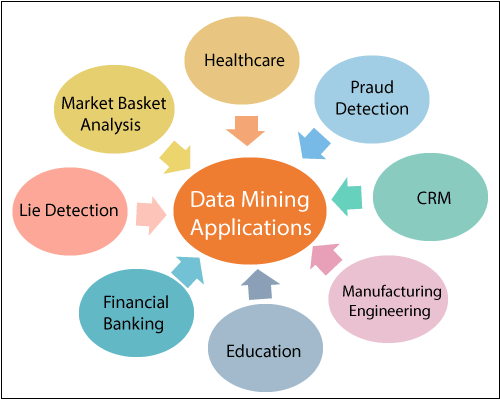
\includegraphics[width=\linewidth]{DApp.png}
\end{figure}
These are the following areas where data mining is widely used:
\subsection{Data Mining in Healthcare:}

Data mining in healthcare has excellent potential to improve the health system. It uses data and analytics for better insights and to identify best practices that will enhance health care services and reduce costs. Analysts use data mining approaches such as Machine learning, Multi-dimensional database, Data visualization, Soft computing, and statistics. Data Mining can be used to forecast patients in each category. The procedures ensure that the patients get intensive care at the right place and at the right time. Data mining also enables healthcare insurers to recognize fraud and abuse.
\subsection{Data Mining in Market Basket Analysis:}

Market basket analysis is a modeling method based on a hypothesis. If you buy a specific group of products, then you are more likely to buy another group of products. This technique may enable the retailer to understand the purchase behavior of a buyer. This data may assist the retailer in understanding the requirements of the buyer and altering the store's layout accordingly. Using a different analytical comparison of results between various stores, between customers in different demographic groups can be done.

\subsection{Data Mining in Education:}

Education data mining is a newly emerging field, concerned with developing techniques that explore knowledge from the data generated from educational Environments. EDM objectives are recognized as affirming student's future learning behavior, studying the impact of educational support, and promoting learning science. An organization can use data mining to make precise decisions and also to predict the results of the student. With the results, the institution can concentrate on what to teach and how to teach

\subsection{Data Mining in Manufacturing Engineering:}

Knowledge is the best asset possessed by a manufacturing company. Data mining tools can be beneficial to find patterns in a complex manufacturing process. Data mining can be used in system-level designing to obtain the relationships between product architecture, product portfolio, and data needs of the customers. It can also be used to forecast the product development period, cost, and expectations among the other tasks
\newpage
\subsection{Data Mining in CRM (Customer Relationship Management):}

Customer Relationship Management (CRM) is all about obtaining and holding Customers, also enhancing customer loyalty and implementing customer-oriented strategies. To get a decent relationship with the customer, a business organization needs to collect data and analyze the data. With data mining technologies, the collected data can be used for analytics.

\subsection{Data Mining in Fraud detection:}

Billions of dollars are lost to the action of frauds. Traditional methods of fraud detection are a little bit time consuming and sophisticated. Data mining provides meaningful patterns and turning data into information. An ideal fraud detection system should protect the data of all the users. Supervised methods consist of a collection of sample records, and these records are classified as fraudulent or non-fraudulent. A model is constructed using this data, and the technique is made to identify whether the document is fraudulent or not

\subsection{Data Mining in Lie Detection:}


Apprehending a criminal is not a big deal, but bringing out the truth from him is a very challenging task. Law enforcement may use data mining techniques to investigate offenses, monitor suspected terrorist communications, etc. This technique includes text mining also, and it seeks meaningful patterns in data, which is usually unstructured text. The information collected from the previous investigations is compared, and a model for lie detection is constructed.

\subsection{Data Mining Financial Banking:}

The Digitalization of the banking system is supposed to generate an enormous amount of data with every new transaction. The data mining technique can help bankers by solving business-related problems in banking and finance by identifying trends, casualties, and correlations in business information and market costs that are not instantly evident to managers or executives because the data volume is too large or are produced too rapidly on the screen by experts. The manager may find these data for better targeting, acquiring, retaining, segmenting, and maintain a profitable customer

\end{document}